\documentclass{beamer}
\usepackage[utf8]{inputenc}
\usepackage{caption}
\usepackage{subcaption}

\title{Strategies for computing the scalar self-force on a Schwarzschild background}
\author{Steven Dorsher}
\institute{Louisiana State University}
\date{September 26, 2017}

\begin{document}
\frame{\titlepage}


\begin{frame}
  \frametitle{Overview}
  \begin{itemize}
  \item Gravitational waves and Extreme Mass Ratio Inspirals
  \item The wave equation in flat spacetime
  \item Scalar waves on a Schwarzschild background without a source
  \item A scalar source on a Schwarzshild background on a circular orbit
  \item A scalar source on a Schwarzschild background on an eccentric orbit
  \item First order Richardson extrapolation
  \item The Discontinuous Galerkin method
  \item Fit to extend the mode sum to $\ell=\infty$
  \item Future work: a comparison of the self-consistent evolution and the geodesic evolution
  \end{itemize}
\end{frame}


\begin{frame}
  \frametitle{Extreme Mass Ratio Inspirals}
  \begin{figure}
    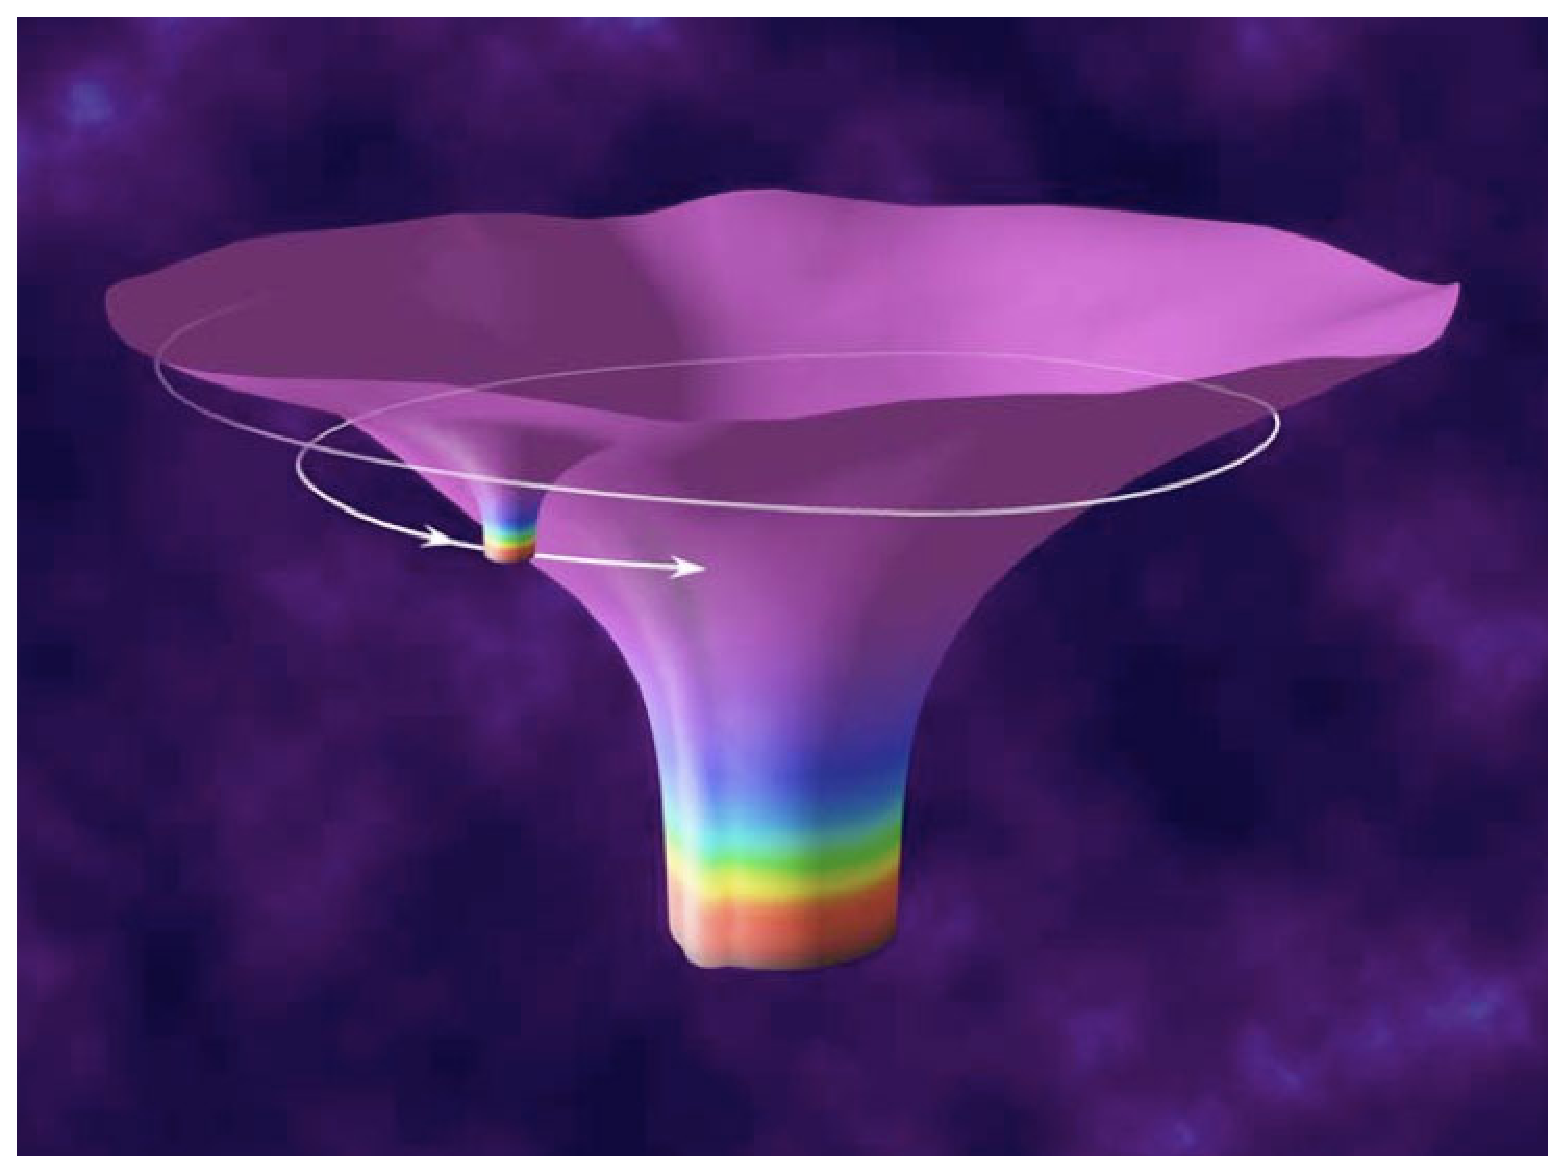
\includegraphics[width=4.0in]{EMRI}
    \citation{Extreme Mass Ratio Inspiral, $\mu=m/M\sim 10^{-4}$ to $10^{-6}$, Artist's rendition, Wikipedia}
  \end{figure}
\end{frame}

\begin{frame}
  \frametitle{Laser Interferometer Space Antenna}
  \begin{figure}
    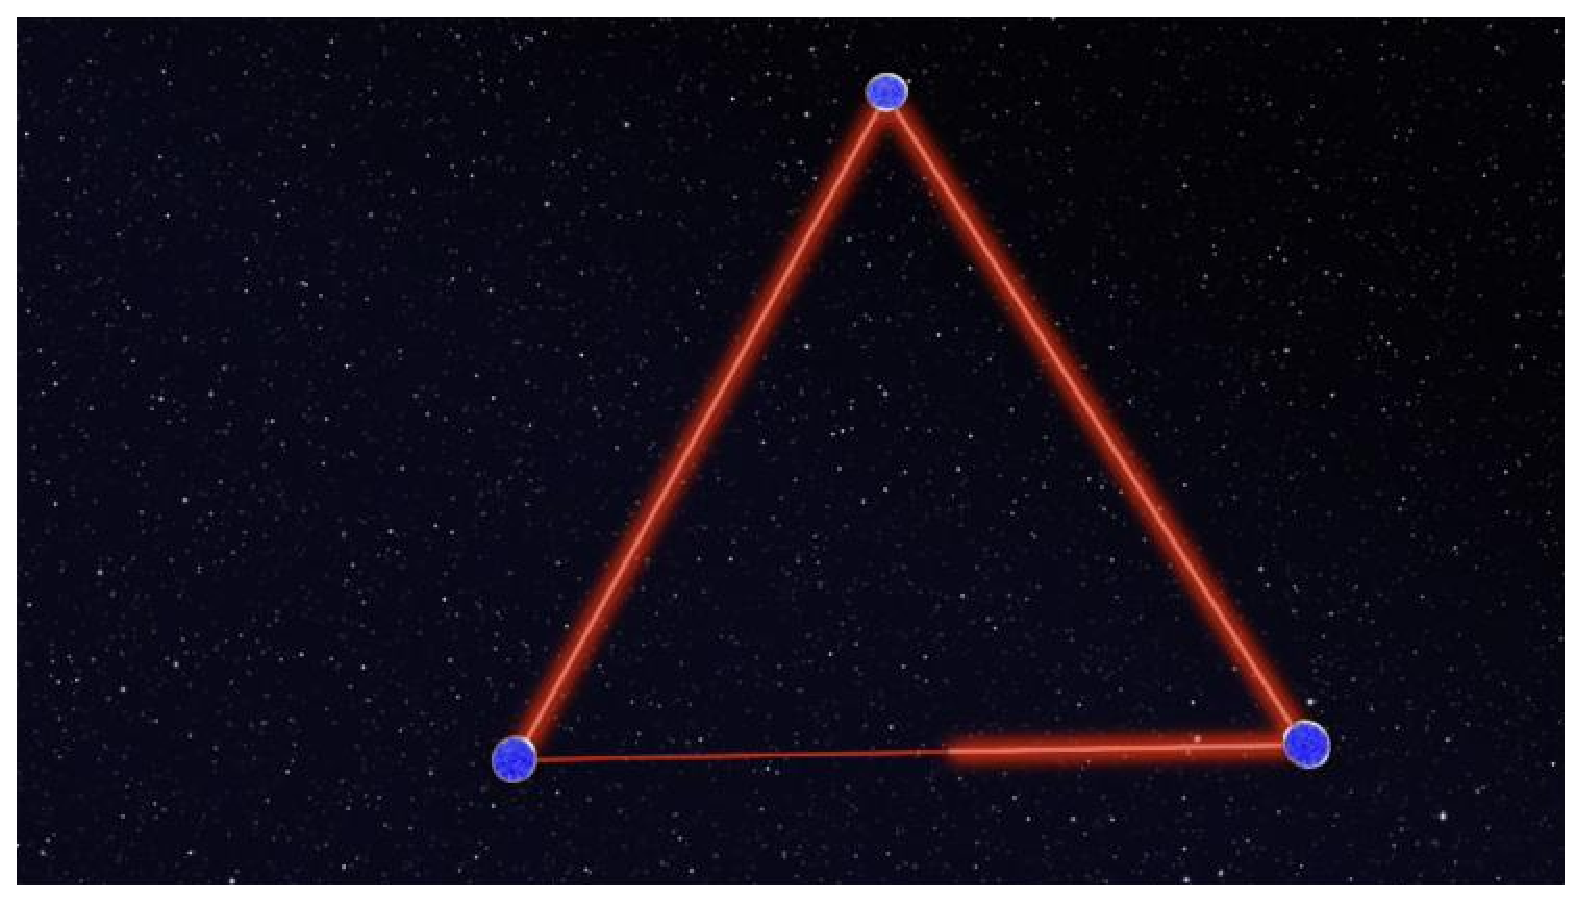
\includegraphics[width=4.0in]{eLISA}
    \caption{Laser Interferometer Space Antenna, which will operate around launches in early 2030's, ESA-NASA partnership, will detect EMRI's}
  \end{figure}
\end{frame}


\begin{frame}
  \frametitle{Gravitational Waves}
  \begin{figure}
    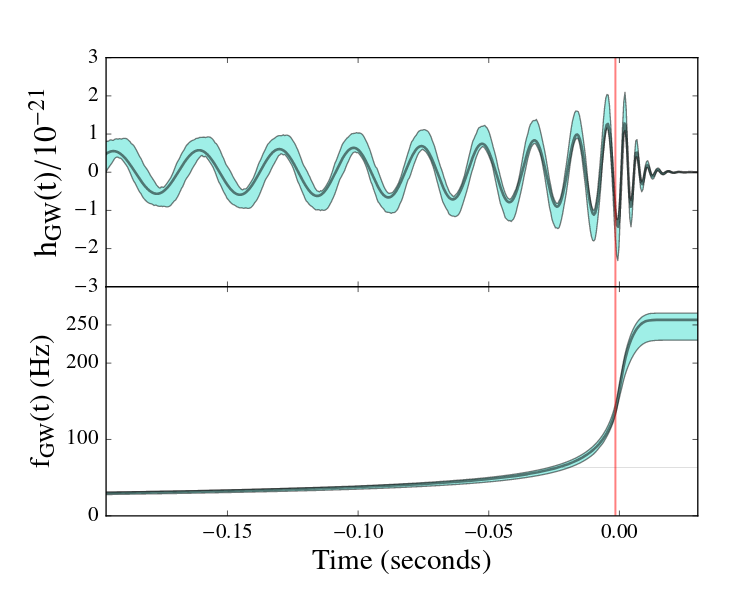
\includegraphics[width=3.0in]{LIGOGRtest.png}
    \caption{LIGO detection, September 14, 2015. General relativity was tested by comparing inpsiral with merger/ringdown phases.}
  \end{figure}
\end{frame}

\begin{frame}
  \frametitle{Self-force}
  \begin{itemize}
  \item The self-force is a particle's interaction with its own field
  \item Applies to scalar, electromagnetic, and tensor fields on a gravitational background
  \item Motion $\rightarrow$ radiation $\rightarrow$ energy and angular momentum loss $\rightarrow$ inspiral
  \item Electromagnetic or gravitational field: source from perturbation theory
  \item Scalar: delta function source
  \end{itemize}
\end{frame}

\begin{frame}
  \frametitle{Approximations and Goals}
  The long term goal for the field is to generate extremely precise EMRI gravitational wave templates for LISA.

  Approximations:
  \begin{itemize}
  \item Scalar rather than tensor waves ($\Psi$ rather than $h_{\mu\nu}$)
  \item Non-rotating black holes: Schwarzschild spacetime
  \item 4D spacetime: time $+$ radius $+$ spherical harmonics
  \item Discontinuous Galerkin spatial grid
  \item Self-force causes a particle to inspiral as it emits radiation
  \item We use the Detweiler-Whiting effective source as implemented by Barry Wardell
  \item Niels Warburton assumes: the particle has been on the same geodesic for all time when he calculates the self-force
  \end{itemize}
  
  Our goal is to implement a highly accurate self-consistent evolution and do a comparison study with Niels Warburton.
  
\end{frame}


\begin{frame}
  \frametitle{The Discontinuous Galerkin (DG) method}
  \begin{itemize}
  \item Method for solving ODEs dependent on space and time.
  \item Break space into evenly spaced elements.
  \item Within each element there are $N$ unevenly spaced nodes connected by $N+1$ interpolating polynomials.
  \item Allows discontinuities at element boundaries-- numerical fluxes
  \item The DG method returns a derivative matrix that takes a derivative across an element and a lift matrix that accounts for numerical fluxes,
  \item Beneficial because it has truncation error that decreases exponentially with DG order $N$ and because it naturally handles discontinuities in $\phi$ and $\rho$. 
  \end{itemize}
\end{frame}



\begin{frame}
  \frametitle{A simple test of the DG method: a wave equation in flat spacetime}
  For no source, the D'Alembertian equals zero:
  \begin{equation}
    \Box\Psi=0
  \end{equation}
  In 1-dimension:
  \begin{equation}
    \frac{\partial^2\Psi}{\partial t^2}-\frac{\partial^2\Psi}{\partial x^2}=0
  \end{equation}
  Rewrite as ODE
  \begin{eqnarray}
    \partial_t \psi &= \rho\nonumber\\
    \partial_t \rho &= \partial_r \phi\nonumber\\
    \partial_t \phi &= \partial_r \rho
  \end{eqnarray}
  Refer to $u=(\psi,\rho,\phi)$ as the state vector.
\end{frame}

\begin{frame}
  \frametitle{Flat space evolution}
  \begin{figure}
    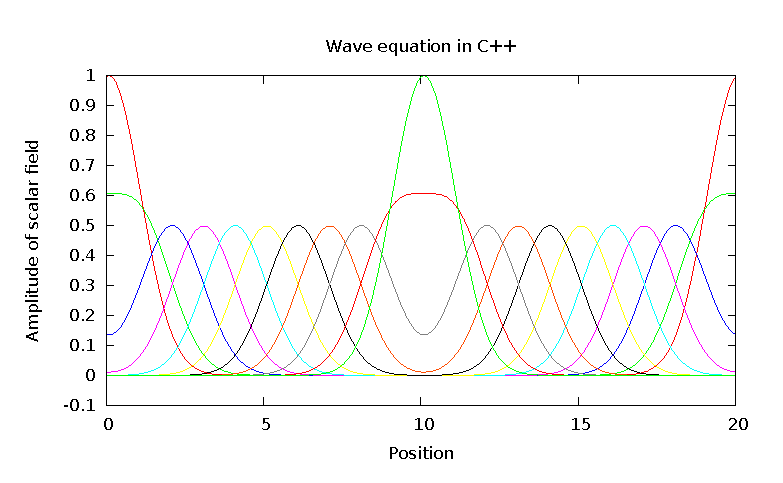
\includegraphics[width=4.0in]{gaussWave}
    \caption{Gaussian initial conditions, flat spacetime}
  \end{figure}
\end{frame}



\begin{frame}
  \frametitle{Flat spacetime error convergence}
  \begin{figure}
    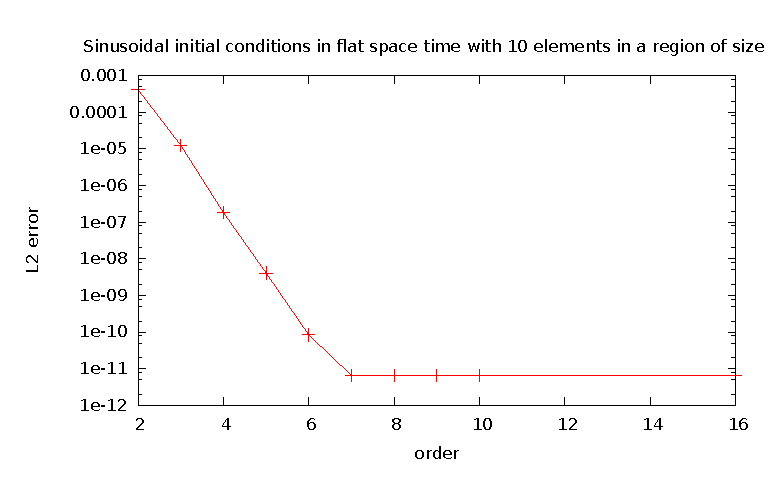
\includegraphics[width=4.0in]{sinL2WTorder}
    \caption{$L_2$ error converges exponentially until it hits roundoff noise with DG order for sinusiodal initial conditions with ten elements of size $h=0.01$.}
  \end{figure}
\end{frame}


\begin{frame}
  \frametitle{Schwarzschild spacetime without a source}
  \begin{itemize}
  \item Wave equation: $\Box\Psi=\partial_\mu\left(\frac{1}{\sqrt{-g}}g^{\mu\nu}\partial_\nu\Psi\right)=0$
  \item Tortoise coordinates in interior
  \item Hyperboloidal coordinates near horizon and at infinity to bring lightlike infinity, $\mathcal{I}^+$, to a finite coordinate
  \item Multipole moment decomposition to account for angular dependence
  \item Expect quasinormal mode ringing with higher frequencies for higher $l$ followed by power law tails that go as $t^{-(2l+3)}$
  \item QNM ringing: interactions near peak of potential
  \item Tails: scattering off spacetime far from peak of potential
  \end{itemize}
\end{frame}

\begin{frame}
  \frametitle{Quasinormal modes}
  \begin{figure}
    \centering
    \begin{subfigure}{.45\textwidth}
      \centering
      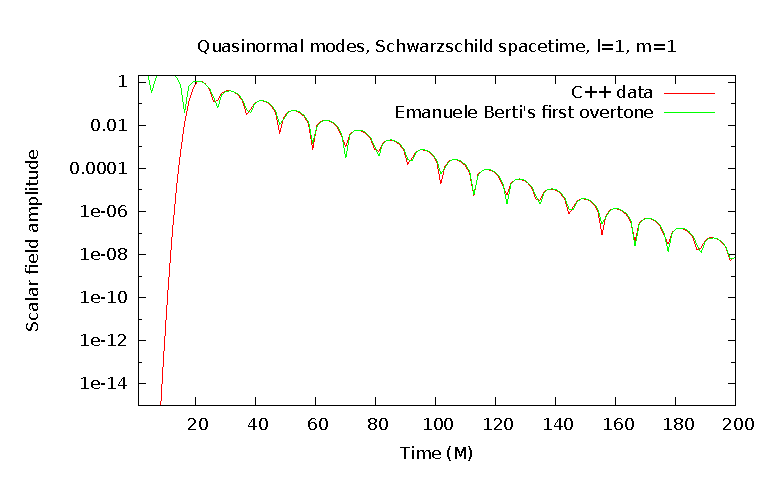
\includegraphics[width=\textwidth]{l1m1qnm}
      \caption{$l=1$}
    \end{subfigure}
    \begin{subfigure}{.45\textwidth}
      \centering
      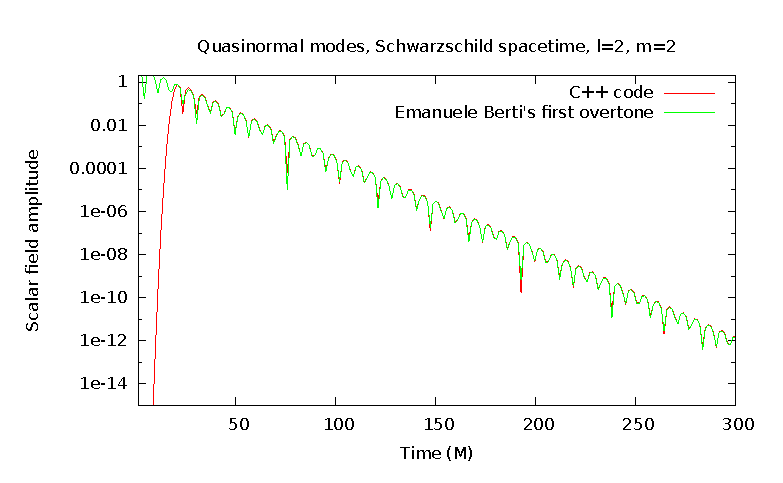
\includegraphics[width=\textwidth]{l2m2qnm}
      \caption{$l=2$}
    \end{subfigure}
  \caption{$l=2$ has a higher frequency and a faster decay rate than $l=1$}
  \end{figure}
\end{frame}

\begin{frame}
  \frametitle{Power law tails}
  \begin{figure}
    \centering
    \begin{subfigure}{.45\textwidth}
      \centering
      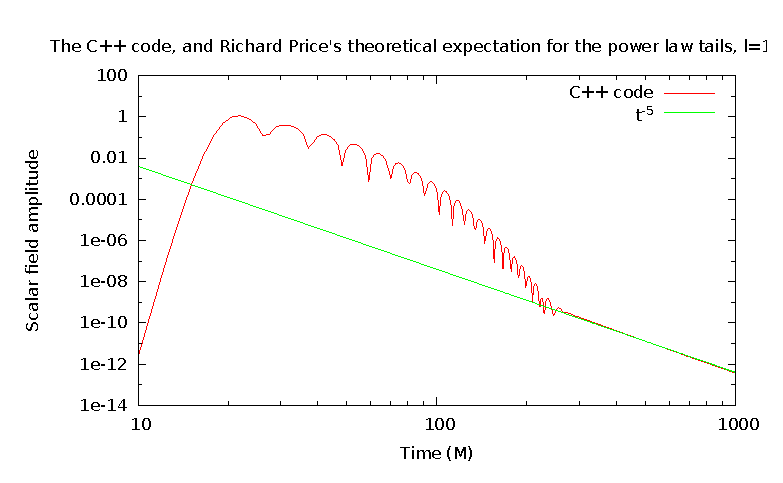
\includegraphics[width=\textwidth]{l1m1tail2}
      \caption{$l=1$}
  \end{subfigure}
    \begin{subfigure}{.45\textwidth}
      \centering
      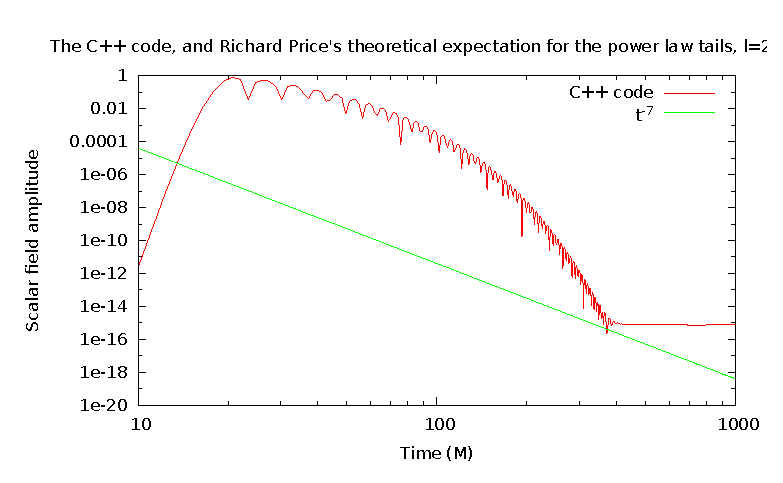
\includegraphics[width=\textwidth]{l2m2tailfail2}
      \caption{$l=2$}
    \end{subfigure}
  \caption{$l=1$ decays as $t^-{-5}$ as expected; however, $l=2$ has no power law tail due to truncation error}
  \end{figure}
\end{frame}



\begin{frame}
  \frametitle{Scalar charge on a circular orbit with an effective source}
  \begin{itemize}
  \item Self-force causes the particle to emit radiation and inspiral. An artifical force holds it on a circular orbit.
  \item Wave equation for retarded field has delta function source proportional to charge
  \item Delta function source is singular
  \item Regularize field: $\Psi^R=\Psi^{ret}-\Psi^S$
  \item Perturbative expansion to Detweiler-Whiting singular field in terms of powers of radius around singular field
  \item Detweiler-Whiting singular field: {\em Steven Detweiler, Bernard F. Whiting (2002). Phys. Rev. D 67, 024025}
  \item Perturbative expansion: {\em Anna Heffernan, Adrian Ottewill, Barry Wardell (2012). Phys. Rev. D 86, 104023}
  \item World tube window function
  \item I have ported this from Fortran to C++ with partially redesigned structure. I have succeeded in reproducing the results to roundoff error precision.  
  \end{itemize}
\end{frame}

\begin{frame}
  \frametitle{Circular orbit roundoff error comparison between languages}
  \begin{figure}
    \centering
    \begin{subfigure}{.45\textwidth}
      \centering
      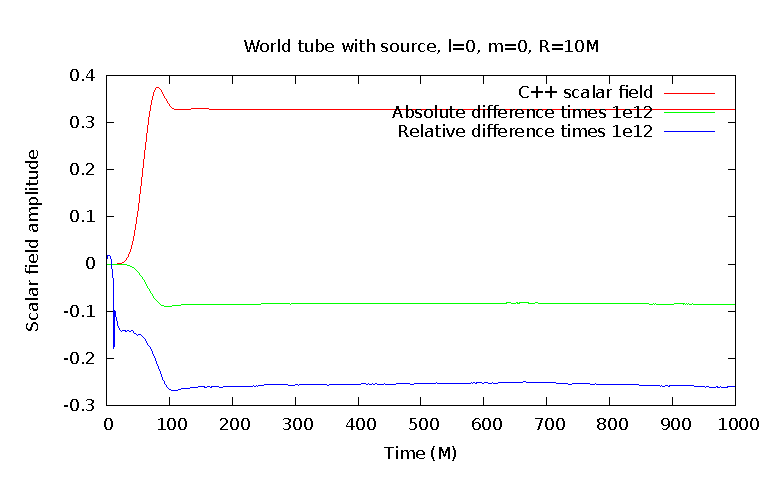
\includegraphics[width=\textwidth]{wtcircl0m0}
      \caption{l=0}
   \end{subfigure}
    \begin{subfigure}{.45\textwidth}
      \centering
      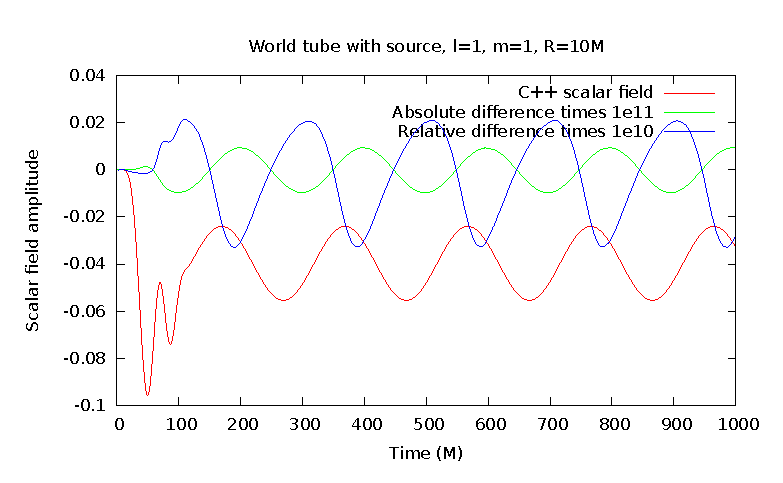
\includegraphics[width=\textwidth]{wtcircl1m1}
      \caption{l=1}
    \end{subfigure}
  \caption{Relative and absolute errors are at the roundoff level-- $10^{-10}$ to $10^{-12}$. Oscillations do not appear in the $l=0$ mode but appear with the orbital period in the $l=1$ mode.}
  \end{figure}
\end{frame}

\begin{frame}
  \frametitle{Eccentric orbits using Peter Diener's simulation}
  \begin{itemize}
  \item Radial oscillations and angular oscillations have different periods
  \item The orbit precesses
  \item The orbit is artifically held on a geodesic to counteract the self-force generating the scalar waves
  \item Oribital parameters can be entirely expressed in terms of $p$, $e$, $\phi$, $\chi$, and $t$.
  \item $r_{periastron}=\frac{pM}{1+e}$, $r_{apastron}=\frac{pM}{1-e}$
  \item A time dependent transformation keeps the particle's coordinate fixed at a Discontinuous Galerkin element boundary
  \item Radial self-force: $F_r=q\partial_r\Psi^R$
  \item Use Niels Warburton's frequency domain initial conditions for $l=0$ through $l=6$. No transients expected in these modes.
  \item Warburton initial conditions: particle has been on the same geodesic for all time
  \item Diener initial conditions: field starts at zero with particle at aphelion
  \end{itemize}
\end{frame}

\begin{frame}
  \frametitle{Precession of the eccentric orbit}
  \begin{figure}
    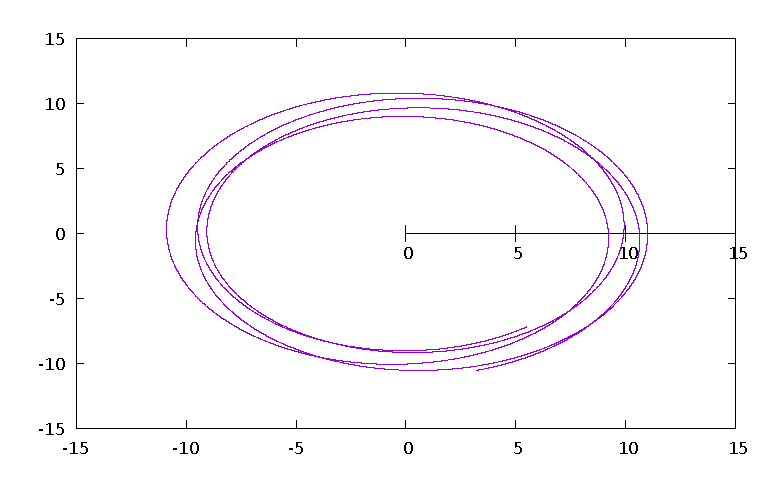
\includegraphics[width=0.9\textwidth]{orbitevolvedg44p99e01}
    \caption{Precession of the eccentric orbit. $p=9.9$, $e=0.0$.}
  \end{figure}
\end{frame}

\begin{frame}
  \frametitle{Evolution of the radial self-force for different initial conditions}
  \begin{figure}
  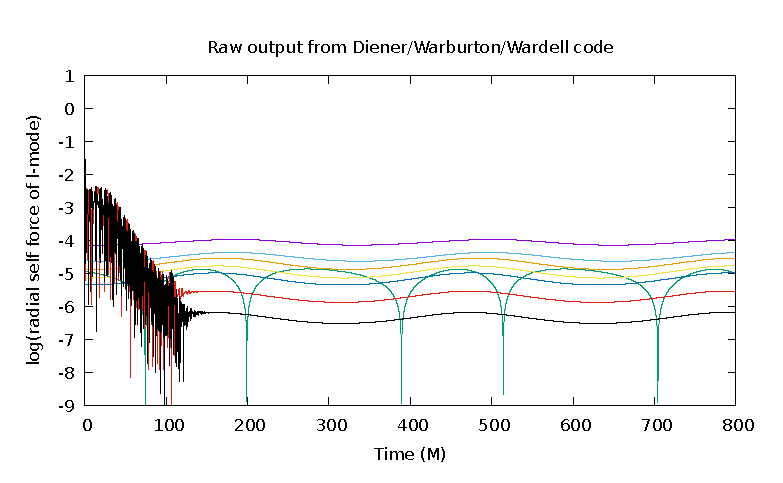
\includegraphics[width=0.9\textwidth]{rawRadialSelForceModes}
  \caption{Modes zero through seven are shown. Zero through five have smooth starts. Six and seven have transients.}
  \end{figure}
\end{frame}

\begin{frame}
  \frametitle{Addressing instabilities and error}
  \begin{itemize}
  \item To address instabilities in accelerated evolutions, I ran eccentric orbits with accelerations of zero.
  \item Analyzed error due to:
    \begin{itemize}
    \item Neglecting the first order Richardson extrapolation
    \item Choice of start and end modes in mode sum fit
    \item Choice of number of terms in mode sum fit
    \item Selection of weights associated with mode sum fit
    \end{itemize}
  \item Concluded the first three errors were comparable and at the $10^{-4}$ level
  \end{itemize}
\end{frame}

\begin{frame}
  \frametitle{The first order Richardson extrapolation}
  \begin{itemize}
  \item Truncation error is skewed entirely to one side when measured using $L_0$ or $L_2$ error
  \item Convergent code approaches an asymptote
  \item Assume $F_r(n,l)=F_{inf}(l)+c(l)\exp(-\alpha n)$
  \item Use three different DG orders $n=n_1$, $n_1+4$, and $n_1+8$ to obtain an extrapolation to $F_{inf}$ from starting order $n_1$
  \item Not all starting orders have solutions because some fail to follow the expected exponential behavior due to roundoff noise-- get NaNs
  \end{itemize}
\end{frame}

\begin{frame}
  \frametitle{Well-converging data}
  \begin{figure}
  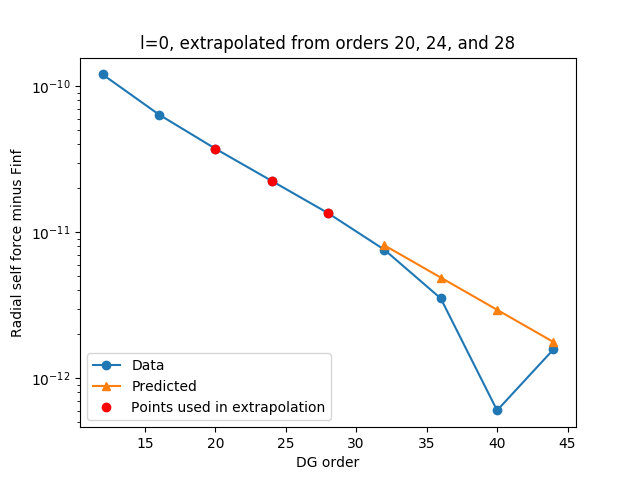
\includegraphics[width=0.9\textwidth]{fittingtechniqet370l0}
  \caption{l=0 at t=370. This data converges very cleanly until it hits roundoff noise at high DG orders.}
  \end{figure}
\end{frame}

\begin{frame}
  \frametitle{Asymptote method for finding the best starting order}
  \begin{itemize}
  \item Might expect second order truncation error to also follow a convergent form on theoretical grounds but data is sparsely populated due to NaN modes
  \item When there are four or five data points, concave. Use first and second derivative test.
  \item When there are fewer, average, then veto one sigma outliers. Average again. Take point closest to second average as best choice.
  \end{itemize}
\end{frame}
  

\begin{frame}
  \frametitle{Error due to neglecting the first order Richardson Extrapolation}
  \begin{figure}
    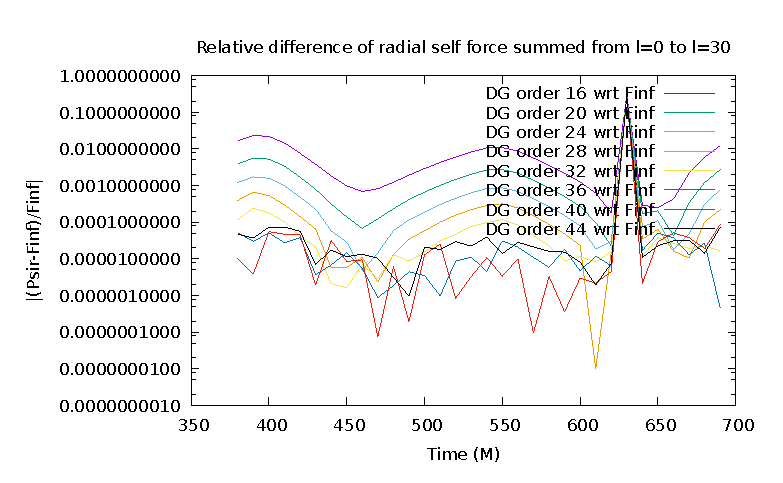
\includegraphics[width=0.9\textwidth]{reldiffpsirvtwfinfdgorders}
    \caption{Relative error between DG starting orders and $F_{inf}$ vs time. For DG order 36 where roundoff error sets in, the error is about $10^{-4}$.}
  \end{figure}
\end{frame}

\begin{frame}
  \frametitle{The l-mode sum and fit}
  \begin{eqnarray}
    F_r(l,t)=&\frac{A(t)}{(2l-1)(21+3)}+\frac{B(t)}{(2l-3)(2l-1)(2l+3)(2l+5)}\nonumber \\
    &+\frac{C(t)}{(2l-5)(2l-3)(2l-1)(2l+3)(2l+5)(2l+7)}+\ldots
  \end{eqnarray}

  {\em Barry Wardell, Ian Vega, Jonathan Thornburg, Peter Diener (2012). Phys. Rev D. 85, 104044}

  \begin{itemize}
  \item Fit from $l_{min}$ to $l_{max}$.
  \item Sum numerically from zero to $l_{max}$ then use fit coefficients to analytically sum to $l=\infty$
  \item Least squares fit: minimize $\chi^2$
  \end{itemize}

  \begin{equation}
    \chi^2=\sum_i\frac{(y_i-f(x_i))^2}{\sigma_i^2}
  \end{equation}

\end{frame}


\begin{frame}
  \frametitle{l-mode fit with three weight models}
  \begin{figure}
    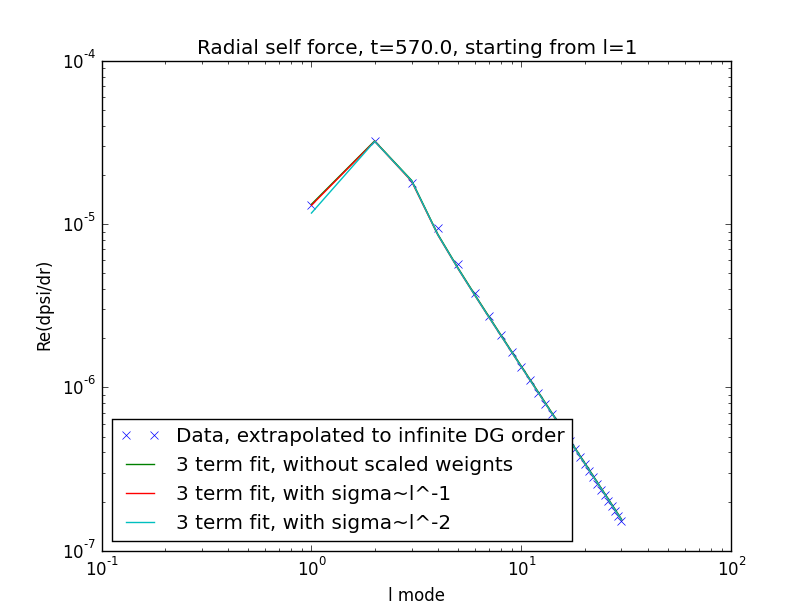
\includegraphics[width=0.9\textwidth]{fiterrscalecorrect3term570l1}
    \caption{l-mode versus $F_{inf}$.}
  \end{figure}
\end{frame}

  
\begin{frame}
  \frametitle{Residuals to the l-mode fit}
  \begin{figure}
    \centering
    \begin{subfigure}{.45\textwidth}
      \centering
      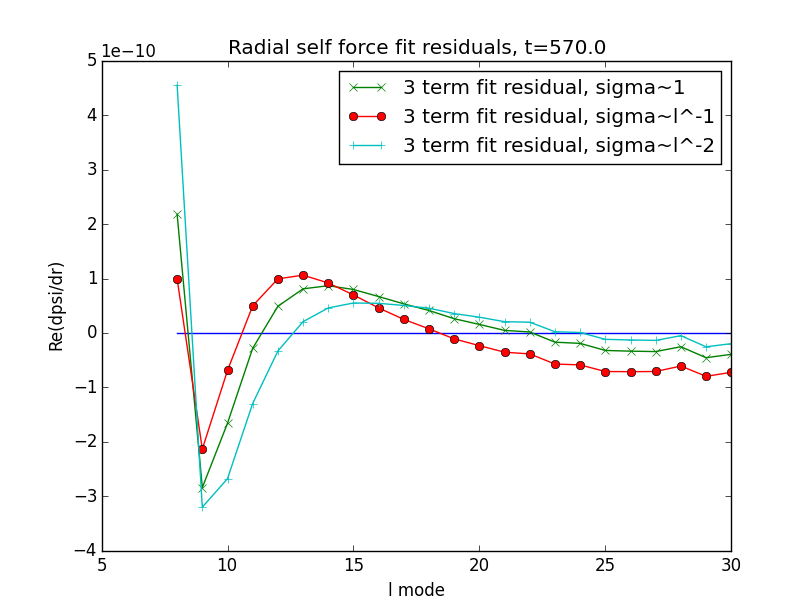
\includegraphics[width=\textwidth]{fitresiduals3terms570l8}
      \caption{$l_{min}=8$}
    \end{subfigure}
    \begin{subfigure}{.45\textwidth}
      \centering
      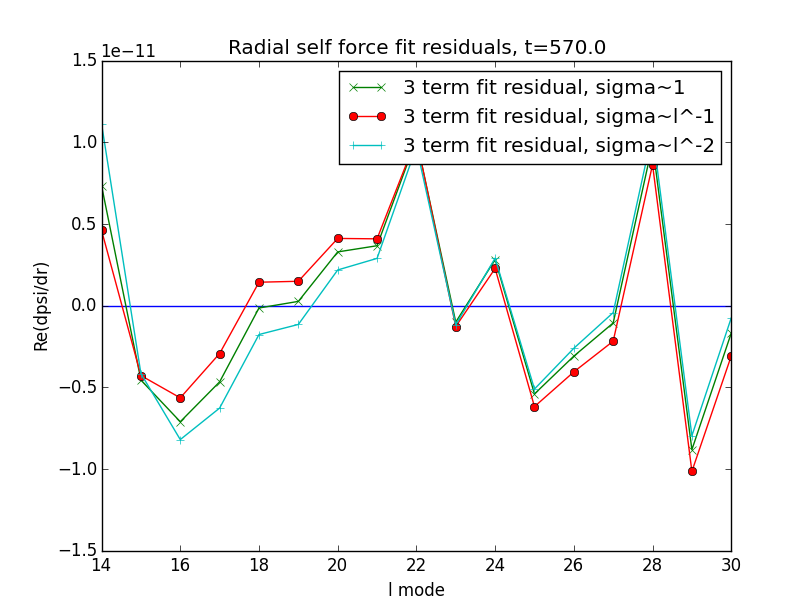
\includegraphics[width=\textwidth]{fitresidulas3terms570l14}
      \caption{$l_{min}=14$}
    \end{subfigure}
  \caption{$l_{min}=14$ is a better fit than $l_{min}=8$ both because it is less systematically biased and because it has an amplitude an order of magnitude smaller. Both fits end at $l_{max}=30$.}
  \end{figure}
\end{frame}

\begin{frame}
  \frametitle{Roundoff noise in $F_{inf}$ at high $l_{max}$}
  \begin{figure}
    \centering
    \begin{subfigure}{.45\textwidth}
      \centering
      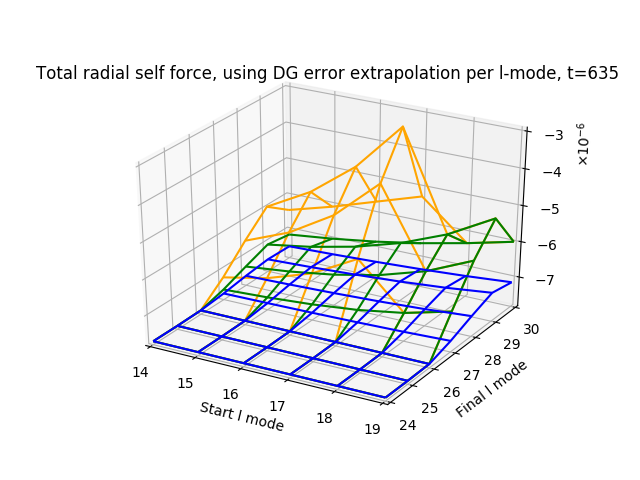
\includegraphics[width=\textwidth]{bestfinflminlmax234terms635fullrange_perihelion}
      \caption{Large range}
    \end{subfigure}
    \begin{subfigure}{.45\textwidth}
      \centering
      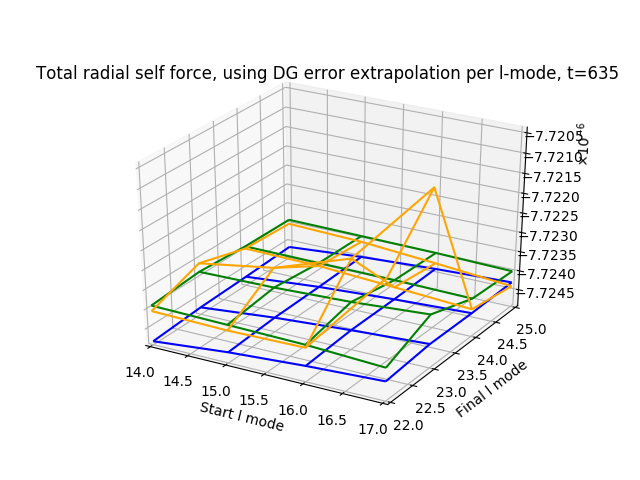
\includegraphics[width=\textwidth]{bestfinflminlmax234termst635smallrange_perihelion}
      \caption{Small range}
    \end{subfigure}
  \caption{$l_{min}=14$ and $l_{max}=25$ appear to be good start and stop values. Roundoff noise is evident at higher l.}
  \end{figure}
\end{frame}

\begin{frame}
  \frametitle{Smooth evolution of total radial self-force}
  \begin{figure}
    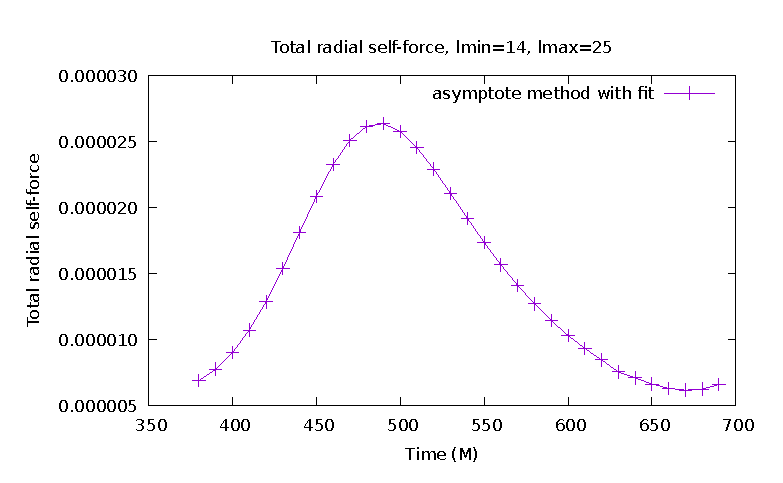
\includegraphics[width=0.9\textwidth]{totalselfforcevt2}
     \caption{Total radial self-force including sum to $l=\infty$ over time}
  \end{figure}
\end{frame}

\begin{frame}
  \frametitle{Error due to l-mode selection, number of terms}
  \begin{figure}
    \centering
    \begin{subfigure}{.45\textwidth}
      \centering
      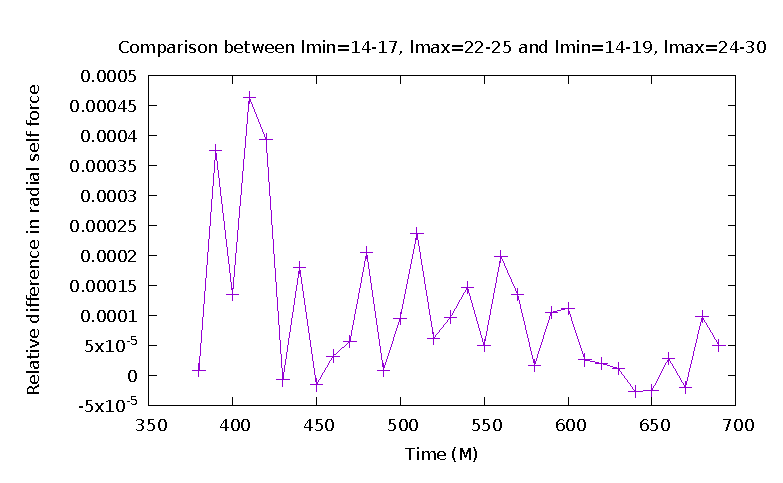
\includegraphics[width=\textwidth]{relErrBigSmallRangeOverTime}
      \caption{large versus small range}
    \end{subfigure}
    \begin{subfigure}{.45\textwidth}
      \centering
      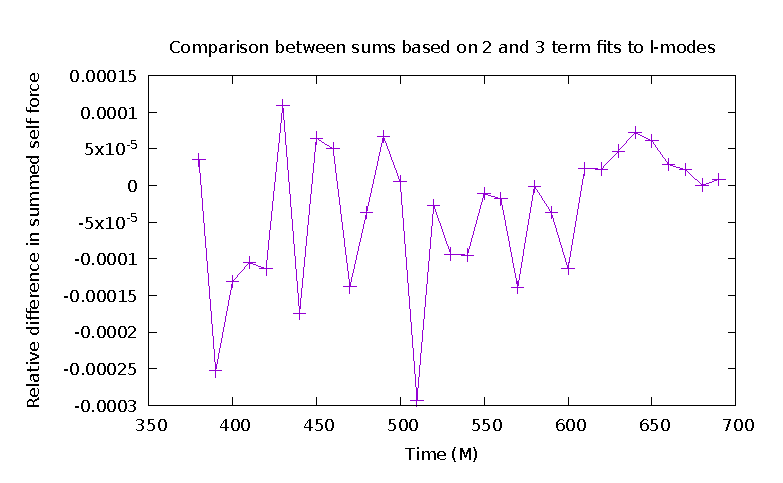
\includegraphics[width=\textwidth]{relativeError23termSelfForce}
      \caption{2 versus 3 terms}
    \end{subfigure}
  \caption{Relative errors in both of these effects appear to be at the $10^{-4}$ level.}
  \end{figure}
\end{frame}

      
\begin{frame}
  \frametitle{Comparison study of self-consistent evolution to geodesic evolution}
  \begin{itemize}
  \item Self-consistent evolution accounts for the interaction of the particle with the field it has generated in the past naturally since it is evolved in the time domain
    \begin{itemize}
    \item Uses the Detweiler-Whiting singular field 
    \item The particle position evolves according to the geodesic equation with an acceleration on the right hand side
    \item The mass of the particle also evolves according to the work being done on it
    \end{itemize}
  \item Geodesic evolution uses an self-force that assumes the particle has been evolving on the same geodesic for all time
    \begin{itemize}
    \item Self-force can be efficiently calculated in the frequency domain due to periodicity
    \item Frequency domain component is good for initial conditions without transients
    \item Evolves in the time domain after generating the self-force in the frequency domain
    \item Cannot handle effects where the timescale of the orbital evolution is short compared to the period
    \end{itemize}
  \end{itemize}
\end{frame}

\begin{frame}
  \frametitle{Long term goals}
  \begin{itemize}
  \item Goal is to compare Diener's self-consistent code using Warburton's initial conditions and Wardell's effective source to Warburton's geodesic evolutions
  \item I will run code, analyze physics, and debug, as necessary.
  \item Timescale: 2-3 years
  \end{itemize}
\end{frame}

\end{document}


  
